% ==============================================================================
% DOCUMENTO DE DISEÑO Y MEMORIA TÉCNICA - ESCAPE CORPORATIVO: LA FUGA DEL EMPLEADO
% Universidad Argentina de la Empresa (UADE) - Paradigma Orientado a Objetos
% ==============================================================================
\documentclass[12pt, a4paper]{article}

% --- Paquetes de codificación e idioma ---
\usepackage[utf8]{inputenc}
\usepackage[T1]{fontenc}
\usepackage[spanish, es-tabla, es-nodecimaldot]{babel}
\usepackage{amsmath}

% --- Tipografía, justificación y sangría en todos los apartados ---
\usepackage{mathptmx} % Fuente Times New Roman estándar académica
\usepackage[top=2.5cm, bottom=2.5cm, left=2.5cm, right=2.5cm]{geometry}
\usepackage{setspace}
\onehalfspacing
\usepackage{indentfirst} % Aplica sangría también al primer párrafo tras cada título
\usepackage{microtype}   % Optimiza el espaciado entre letras para justificación perfecta
\setlength{\parindent}{1.25cm} % Sangría estándar de primera línea (tipo tabulación)
\setlength{\parskip}{0.4em}    % Espaciado suave entre párrafos
\sloppy                        % Evita que palabras técnicas largas sobresalgan del margen derecho

% --- Tablas y colores ---
\usepackage[table]{xcolor}
\usepackage{booktabs}
\usepackage{tabularx}
\usepackage{longtable}
\usepackage{array}

% --- Gráficos, diagramas vectoriales, código y enlaces ---
\usepackage{graphicx}
\usepackage{float}
\usepackage{enumitem}
\usepackage{fancyhdr}
\usepackage{titlesec}
\usepackage[hidelinks, colorlinks=true, linkcolor=black, urlcolor=blue]{hyperref}

% --- Definición de colores institucionales y de tabla ---
\definecolor{headerbg}{HTML}{F0EEF6}
\definecolor{bordergray}{HTML}{D3D3D3}
\definecolor{codegreen}{HTML}{1E6B3A}
\definecolor{uadeblue}{HTML}{1B365D}

% --- Comando para formatear nombres de clases, métodos y símbolos de código ---
% Habilita la separación automática en fuente monoespaciada (\texttt) sin romper macros
\DeclareRobustCommand{\code}[1]{\textcolor{codegreen}{\texttt{\hyphenchar\font=`\-#1}}}

% --- Configuración de encabezados y pies de página ---
\pagestyle{fancy}
\fancyhf{}
\renewcommand{\headrulewidth}{0pt}
\fancyfoot[R]{\thepage}

% --- Formato de títulos de secciones (con sangría activa en el párrafo siguiente) ---
\titleformat{\section}
  {\normalfont\large\bfseries\centering}{\thesection.}{0.5em}{}
\titleformat{\subsection}
  {\normalfont\normalsize\bfseries\itshape}{\thesubsection.}{0.5em}{}
\titlespacing*{\section}{0pt}{1.5ex plus 0.5ex minus .2ex}{1.0ex plus .2ex}
\titlespacing*{\subsection}{0pt}{1.2ex plus 0.4ex minus .2ex}{0.6ex plus .2ex}

% --- Espaciado de tablas ---
\renewcommand{\arraystretch}{1.5}
\setlength{\tabcolsep}{8pt}

\begin{document}

% ==============================================================================
% 1. ENCABEZADO INSTITUCIONAL Y ACADÉMICO (PORTADA)
% ==============================================================================
\begin{titlepage}
    \centering
    \vspace*{2cm}

    {\Large \textbf{UNIVERSIDAD ARGENTINA DE LA EMPRESA}}\\[0.5cm]
    {\large Ingeniería en Informática}\\[1.5cm]

    {\Large \textbf{PARADIGMA ORIENTADO A OBJETOS (3.4.208)}}\\[0.4cm]
    {\large Trabajo Práctico Obligatorio — Entrega Final}\\[2cm]

    {\huge \textbf{ESCAPE CORPORATIVO: LA FUGA}}\\[0.4cm]
    {\huge \textbf{DEL EMPLEADO}}\\[1cm]

    {\normalsize \textit{Videojuego de acción y estrategia 2D en tiempo real}}\\[2cm]

    {\normalsize Documento de Diseño de Juego, Memoria Técnica y Diagramas UML}\\[0.8cm]

    {\normalsize \textbf{Equipo:} El One Piece (Grupo 1)}\\[0.3cm]
    {\normalsize \textbf{Integrantes:} Alcaide, Yamil; Esponda, Emiliano; Miguez, Ian Franco;\\ Torres, Matías; Villavedra, Santiago Martín}\\[0.6cm]

    {\normalsize \textbf{Profesor:} Hernández, Pablo Eduardo}\\[0.6cm]
    {\normalsize \textbf{Fecha de entrega:} 16/11/2026}

    \vfill
\end{titlepage}

% ==============================================================================
% ÍNDICE DE CONTENIDOS
% ==============================================================================
\newpage
\setcounter{page}{2}
\renewcommand{\contentsname}{}
\vspace*{-1.5cm}
\tableofcontents
\newpage

% Configura la sangría de primera línea (1.25cm) en todo el cuerpo del documento
\setlength{\parindent}{1.25cm}

% ==============================================================================
% 1. INTRODUCCIÓN
% ==============================================================================
\section{Introducción}

\indent El proyecto \textbf{ESCAPE CORPORATIVO: LA FUGA DEL EMPLEADO} consiste en el diseño e implementación de un videojuego 2D de acción y estrategia en tiempo real desarrollado íntegramente en Java. La premisa narrativa posiciona al jugador en el rol de un empleado exhausto que intenta escapar de un entorno de oficina opresivo antes de que venza su horario laboral reglamentario (60 segundos por nivel), mientras evade incansablemente a su Jefe, quien patrulla el sector superior e intenta asignarle horas extra arrojándole proyectiles cargados de tareas (palas).

\indent Desde el punto de vista académico, este desarrollo constituye un caso de estudio práctico para la aplicación genuina e integral de los contenidos de la asignatura \textit{Paradigma Orientado a Objetos (POO)} (Unidades 1 a 6). La arquitectura se estructura bajo el patrón \textbf{MVC (Modelo-Vista-Controlador)}, incorporando abstracción mediante las jerarquías \code{EntidadMovil} y \code{EntidadEstatica}, herencia y polimorfismo para la gestión de actores y potenciadores (\code{Buffo}: \code{Cafe}, \code{Aguinaldo} y \code{Corazon}), e interfaces (\code{IColisionable}, \code{Buffo}, \code{Comparable}, \code{Comparator}, \code{Serializable}, \code{Runnable}) para el desacoplamiento de contratos. Adicionalmente, el sistema implementa principios \textbf{SOLID} y patrones \textbf{GRASP}, colecciones genéricas (\code{ArrayList}, \code{HashMap}, \code{LinkedHashSet}) recorridas con iteradores y bucles \textit{for-each}, una jerarquía de excepciones personalizadas (\textit{checked} y \textit{unchecked}), ejecución multihilo (\code{Thread} y \code{javax.swing.Timer}), persistencia de archivos binarios y de texto plano, y una interfaz gráfica \textit{arcade} construida con Java Swing/AWT que incluye un selector modal de niveles con desbloqueo progresivo.

% ==============================================================================
% 2. OBJETIVO DEL JUEGO
% ==============================================================================
\section{Objetivo del juego}

\indent El objetivo central del jugador consiste en guiar al \code{Empleado} desplazándose en cuatro direcciones cardinales (izquierda, derecha, arriba, abajo) mediante las teclas \texttt{WASD} o flechas direccionales desde su punto de origen en la oficina hasta la \textbf{Salida Principal} de la corporación (\code{Salida}), atravesando una secuencia progresiva de 4 niveles laberínticos con dificultad incremental, muros infranqueables (\code{Muro}), recolectando potenciadores estratégicos (\code{Cafe}, \code{Aguinaldo} y \code{Corazon}) y esquivando los proyectiles lanzados por el \code{Jefe}.

\subsection{Condiciones de victoria}
\begin{itemize}[leftmargin=1.5cm]
    \item El jugador alcanza y superpone su caja de colisión (\code{Posicion}) con las coordenadas de la \textbf{Salida Principal} (\code{Salida.esAlcanzada()}) antes de que finalice la jornada laboral de 60 segundos (\code{EstadoJuego.VICTORIA}).
    \item Al superar un nivel, el sistema calcula una bonificación de puntaje (\code{calcularBonificacionVictoria()}) compuesta por una base de escape (\texttt{500 pts}), el tiempo sobrante ($\text{segundos restantes} \times 10$), las vidas conservadas ($\text{corazones restantes} \times 100$) y un bono adicional (\texttt{+250 pts}) si el empleado cruza la salida conservando su escudo activo (\code{tieneEscudo()}). Asimismo, desbloquea progresivamente el nivel superado en el selector de niveles y habilita el avance al siguiente mapa hasta completar los 4 niveles del juego, mostrar la pantalla final (\code{PanelVictoria}) y registrar el récord consolidado en el Top 10.
\end{itemize}

\subsection{Condiciones de derrota}
\begin{itemize}[leftmargin=1.5cm]
    \item \textbf{Agotamiento de corazones (\code{EstadoJuego.DERROTA\_VIDA}):} El empleado inicia la partida con una reserva global de \textbf{3 corazones} (\code{SALUD\_DEFAULT = 3}) que se conserva a lo largo de los 4 niveles. Cuando un proyectil (\code{Proyectil}) lanzado por el Jefe impacta contra el Empleado (\code{recibirImpacto()}):
    \begin{itemize}[leftmargin=1.0cm]
        \item Si el empleado posee un \textbf{Escudo Protector (\code{Aguinaldo})} activo, el escudo absorbe el impacto y se rompe (\code{Aguinaldo.romper()}), evitando la pérdida de corazones y manteniendo su posición en el mapa.
        \item Si no posee escudo activo, el empleado pierde \texttt{1 corazón}. Si aún conserva corazones disponibles ($2$ o $1$), es devuelto inmediatamente a la coordenada de inicio del nivel (\code{volverAPosicionInicial()}) mientras el reloj de 60 segundos continúa corriendo. Cuando pierde su tercer y último corazón (\code{salud == 0}), la partida concluye en \textit{Game Over}.
    \end{itemize}
    \item \textbf{Vencimiento del horario laboral (\code{EstadoJuego.DERROTA\_TIEMPO}):} El cronómetro de la jornada alcanza el tiempo límite reglamentario (\code{DURACION\_JORNADA\_SEGUNDOS = 60}) sin que el Empleado haya alcanzado la puerta de salida.
\end{itemize}

% ==============================================================================
% 3. ACTORES Y ENTIDADES DEL SISTEMA
% ==============================================================================
\section{Actores y entidades del sistema}

\indent A continuación se detallan los elementos activos y pasivos dentro del dominio del problema (paquetes \code{modelo.entidades} y \code{modelo.items}), clasificados según su responsabilidad e interacción dentro de la simulación.

\subsection{El Empleado}

\indent El jugador interactúa directamente con la clase \code{Empleado} (subclase de \code{EntidadMovil}), administrando sus corazones de vida, su estado de escudo protector, su coordenada de origen en el nivel (\code{xInicial}, \code{yInicial}), su dirección vectorial y la lista de modificadores (\code{List<Buffo>}) recolectados en el mapa.

\begin{table}[H]
\centering
\begin{tabularx}{\textwidth}{>{\raggedright\arraybackslash}p{3.2cm} >{\raggedright\arraybackslash}p{3.8cm} X}
\rowcolor{headerbg}
\textbf{Entidad} & \textbf{Rol} & \textbf{Comportamiento} \\
\hline
\code{Empleado} & Personaje Principal (Avatar) & Movido por el jugador vía teclado en cuatro direcciones (\code{Direccion}). Evalúa colisiones preventivas contra la lista de \code{Muro} antes de consolidar su movimiento, gestiona su reserva de \texttt{3 corazones} (\code{SALUD\_DEFAULT = 3}), su escudo protector (\code{tieneEscudo}), el retorno al punto de partida tras recibir un impacto sin escudo (\code{volverAPosicionInicial()}) y actualiza en cada ciclo el tiempo de vida de sus \code{Buffo} activos mediante un \code{Iterator}. \\
\hline
\end{tabularx}
\end{table}

\subsection{El Jefe y sus Proyectiles}

\indent El \code{Jefe} actúa como el antagonista principal impulsado por un algoritmo de seguimiento autónomo en el pasillo superior, incrementando su cadencia de fuego a medida que el jugador avanza por los 4 niveles.

\begin{table}[H]
\centering
\begin{tabularx}{\textwidth}{>{\raggedright\arraybackslash}p{3.2cm} >{\raggedright\arraybackslash}p{3.8cm} X}
\rowcolor{headerbg}
\textbf{Entidad} & \textbf{Rol} & \textbf{Comportamiento} \\
\hline
\code{Jefe} & Antagonista / IA & Persigue horizontalmente al Empleado a velocidad constante (\code{velocidad = 1}) calculando la diferencia entre los centros geométricos de sus hitboxes (\code{seguirEmpleado()}). Dispara periódicamente con cadencia incremental según el nivel (\texttt{2200 ms} en Nivel 1, \texttt{1850 ms} en Nivel 2, \texttt{1550 ms} en Nivel 3 y \texttt{1250 ms} en Nivel 4). \\
\arrayrulecolor{bordergray}\hline
\code{Proyectil} (Pala / Tarea) & Obstáculo Móvil Balístico & Subclase de \code{EntidadMovil} que implementa \code{IColisionable}. Es instanciado por el Jefe con dirección descendente (\code{Direccion.ABAJO}) y velocidad \texttt{3}. Al impactar al Empleado, reproduce audio asíncrono, rompe el escudo activo o descuenta \texttt{1 corazón} devolviendo al jugador al inicio del nivel, dispara \code{ImpactoProyectilException} y se desactiva (\code{impacto()}). \\
\arrayrulecolor{black}\hline
\end{tabularx}
\end{table}

\subsection{El Entorno (El Laberinto)}

\indent El mapa define los límites físicos del juego y el espacio euclidiano bidimensional (grilla de celdas de $32 \times 32$ píxeles) donde ocurren las colisiones contra las subclases de \code{EntidadEstatica} que implementan \code{IColisionable}.

\begin{table}[H]
\centering
\begin{tabularx}{\textwidth}{>{\raggedright\arraybackslash}p{3.2cm} >{\raggedright\arraybackslash}p{3.8cm} X}
\rowcolor{headerbg}
\textbf{Entidad} & \textbf{Rol} & \textbf{Comportamiento} \\
\hline
Mapa / Grid (\code{char[][]}) & Estructura de Nivel & Matriz bidimensional de caracteres cargada dinámicamente por \code{GestorArchivos} desde \texttt{assets/mapas/nivel\_N.txt} (\texttt{\#} Muro, \texttt{E} Empleado, \texttt{J} Jefe, \texttt{S} Salida, \texttt{C} Café, \texttt{A} Aguinaldo, \texttt{V} Corazón). \\
\arrayrulecolor{bordergray}\hline
\code{Muro} & Obstáculo Rígido & Subclase de \code{EntidadEstatica} que implementa \code{IColisionable}. Bloquea el paso del Empleado impidiendo el solapamiento geométrico de sus cajas envolventes. \\
\hline
\code{Salida} & Punto de Control / Meta & Subclase de \code{EntidadEstatica} que implementa \code{IColisionable}. Define la coordenada de escape y evalúa la condición de victoria (\code{esAlcanzada()}). \\
\hline
\code{ZonaBuffo} & Punto de Obtención de Buffos & Subclase de \code{EntidadEstatica} que implementa \code{IColisionable} y compone una instancia polimórfica de \code{Buffo} (\code{Cafe}, \code{Aguinaldo} o \code{Corazon}). Al colisionar con el jugador, entrega el potenciador (\code{consumirBuffo()}) y se marca como recolectada (con preservación inteligente en piso si el jugador tiene la vida llena al pisar un \code{Corazon}). \\
\arrayrulecolor{black}\hline
\end{tabularx}
\end{table}

% ==============================================================================
% 4. REGLAS DE JUGABILIDAD Y MECÁNICAS
% ==============================================================================
\section{Reglas de jugabilidad y mecánicas}

\indent La lógica del juego se articula a través de tres reglas de negocio centrales traducidas a estructuras del lenguaje Java dentro del motor \code{JuegoEngine}:

\subsection*{Regla 1 — Movimiento, Colisiones y Sistema de 3 Corazones (Motor de Física 2D)}
\indent En cada ciclo del bucle de juego (\texttt{60 FPS}, cada \texttt{16 ms}), la posición tentativa del \code{Empleado} en cuatro direcciones (\code{Direccion.ARRIBA}, \code{ABAJO}, \code{IZQUIERDA}, \code{DERECHA}) se calcula multiplicando el vector unitario $(\text{dx}, \text{dy})$ del enumerador por la velocidad actual. Antes de actualizar las coordenadas $(x_1, y_1, x_2, y_2)$ del objeto \code{Posicion}, se verifica la intersección de cajas envolventes (\textit{Axis-Aligned Bounding Boxes}) mediante el contrato \code{IColisionable.verificarColision()}. Si existe solapamiento con algún \code{Muro}, el desplazamiento se anula. Por su parte, los proyectiles viajan aéreamente en línea descendente y, al solaparse con el hitbox del Empleado, notifican el impacto mediante \code{ImpactoProyectilException}: si el jugador posee escudo (\code{Aguinaldo}), éste absorbe el golpe y se rompe; de lo contrario, pierde 1 corazón y retrocede a la casilla inicial del mapa (\code{volverAPosicionInicial()}) limpiando los proyectiles en vuelo, o cae derrotado (\code{DERROTA\_VIDA}) al perder los 3 corazones.

\subsection*{Regla 2 — Sistema de Buffos (Polimorfismo)}
\indent Todos los potenciadores implementan la interfaz \code{Buffo}, la cual define el contrato polimórfico \code{aplicar(Empleado)}, \code{remover(Empleado)}, \code{actualizar(long)} y \code{estaExpirado()}. Al entrar en contacto con una \code{ZonaBuffo} activa:
\begin{itemize}[leftmargin=1.5cm]
    \item \textbf{\code{Cafe} (\texttt{'C'}):} Incrementa temporalmente la velocidad de desplazamiento del Empleado en \texttt{+3} unidades durante \texttt{5000 ms} (\texttt{5 segundos}) y suma \texttt{50 puntos}. Al expirar su temporizador interno, revierte automáticamente la velocidad a su valor original.
    \item \textbf{\code{Aguinaldo} (\texttt{'A'} — Escudo Protector):} Otorga al Empleado un escudo protector activo (\code{setTieneEscudo(true)}), representado visualmente con un aura cian translúcida alrededor del personaje, capaz de absorber \texttt{1 impacto} de proyectil antes de romperse (\code{romper()}), además de otorgar un bono directo de \texttt{+500 puntos}.
    \item \textbf{\code{Corazon} (\texttt{'V'} — Vida Extra):} Efecto instantáneo que restaura \texttt{+1 corazón} de vida (hasta el tope máximo de \texttt{3 corazones}) y suma \texttt{+100 puntos}. Si el empleado ya cuenta con sus 3 corazones llenos al pisar la casilla, el ítem no se consume en vano y permanece disponible en el piso para cuando sufra daño.
\end{itemize}
\indent Este diseño respeta rigurosamente el principio \textbf{Abierto/Cerrado (OCP)}: el motor y el empleado operan sobre la abstracción \code{Buffo} sin acoplarse a las clases concretas en el ciclo de actualización temporal.

\subsection*{Regla 3 — Progresión Incremental, Selector de Niveles y Persistencia}
\indent El juego estructura su progresión a través de \textbf{4 niveles secuenciales con diseño incremental} (\texttt{nivel\_1.txt} a \texttt{nivel\_4.txt}) administrados por \code{JuegoEngine}:
\begin{itemize}[leftmargin=1.5cm]
    \item \textbf{Nivel 1 (\textit{Primer Paso} — Dificultad Baja):} Corredores amplios de aprendizaje, alta disponibilidad de ayudas (\texttt{3 Cafés}, \texttt{1 Aguinaldo}, \texttt{2 Corazones}) y cadencia de disparo del Jefe de \texttt{2200 ms}.
    \item \textbf{Nivel 2 (\textit{Laberinto Corporativo} — Dificultad Media):} Secciones escalonadas con aberturas alternadas, \texttt{2 Cafés}, \texttt{1 Aguinaldo}, \texttt{2 Corazones} y cadencia de disparo de \texttt{1850 ms}.
    \item \textbf{Nivel 3 (\textit{Ruta Dual} — Dificultad Alta):} Bifurcaciones tácticas con refugios intermedios, \texttt{2 Cafés}, \texttt{1 Aguinaldo}, \texttt{1 Corazón} y cadencia de disparo de \texttt{1550 ms}.
    \item \textbf{Nivel 4 (\textit{El Búnker Central} — Dificultad Extrema):} Cinco barreras horizontales con pasos estrechos en zig-zag bajo fuego intenso, \texttt{2 Cafés}, \texttt{1 Aguinaldo}, \texttt{1 Corazón} y cadencia de disparo de \texttt{1250 ms}.
\end{itemize}
\indent Al superar cada mapa, se consolida el puntaje base, los corazones restantes (\code{corazonesBaseNivelActual}) y el tiempo acumulado, desbloqueando progresivamente dicho nivel en el \textbf{Selector de Niveles Arcade} de \code{PanelInicio} (el cual inicia bloqueado y habilita tarjetas interactivas a medida que el jugador avanza). Si el jugador reintenta un nivel con la tecla \texttt{R}, restaura el puntaje y los corazones exactos con los que ingresó a ese piso. La tabla histórica de los 10 mejores desempeños (\textit{Top 10 High Scores}) se serializa en disco en el archivo binario \texttt{data/ranking.dat} mediante \code{ObjectOutputStream} y \code{ObjectInputStream} dentro del servicio \code{GestorArchivos}.

% ==============================================================================
% 5. MANEJO DE EXCEPCIONES Y EVENTOS
% ==============================================================================
\section{Manejo de Excepciones y Eventos}

\indent El sistema implementa una jerarquía de excepciones personalizadas en el paquete \code{excepciones}, combinando excepciones comprobadas (\textit{checked}), no comprobadas (\textit{unchecked}) y estándar de Java mediante bloques \code{try-catch-finally}, \code{try-with-resources}, \code{throw} y \code{throws} para controlar situaciones anómalas sin interrumpir abruptamente el bucle de ejecución:

\begin{itemize}[leftmargin=1.5cm]
    \item \code{NivelNoEncontradoException} (\textbf{Excepción \textit{checked} que extiende de \code{Exception}}): Declarada con \code{throws} en \code{GestorArchivos.cargarMapaNivel(int)} y lanzada con \code{throw} cuando el archivo de diseño de un nivel (\texttt{nivel\_N.txt}) no existe en el sistema de archivos, se encuentra vacío o sufre un fallo de lectura (\code{IOException}, utilizando constructores sobrecargados con encadenamiento de causa \code{Throwable}). Es capturada en \code{JuegoEngine.cargarNivel()}.
    \item \code{ImpactoProyectilException} (\textbf{Excepción \textit{unchecked} que extiende de \code{RuntimeException}}): Disparada explícitamente en \code{JuegoEngine.actualizarProyectiles()} cuando un \code{Proyectil} colisiona contra la caja envolvente del \code{Empleado}, encapsulando la evaluación de ruptura de escudo o pérdida de corazón, el retroceso a la posición inicial, el disparo de sonido y la transición hacia \code{EstadoJuego.DERROTA\_VIDA} cuando se pierden los 3 corazones.
    \item \textbf{Excepciones estándar y validación de invariantes:} Uso de \code{IllegalArgumentException} ante argumentos inválidos (daño negativo en \code{Empleado.recibirDanio()}, buffo nulo en \code{ZonaBuffo} o puntaje nulo en \code{GestorArchivos.guardarPuntaje()}), y manejo de \code{IOException}, \code{ClassNotFoundException}, \code{FontFormatException}, \code{UnsupportedAudioFileException}, \code{LineUnavailableException} e \code{InterruptedException} con bloques \code{finally} de liberación segura de flujos de audio en \code{GestorAudio.run()}.
\end{itemize}

% ==============================================================================
% 6. ARQUITECTURA TÉCNICA Y DECISIONES DE DISEÑO ORIENTADO A OBJETOS
% ==============================================================================
\section{Arquitectura técnica y decisiones de diseño orientado a objetos}

\subsection{Lenguaje, plataforma y herramientas}
\begin{itemize}[leftmargin=1.5cm]
    \item \textbf{Lenguaje:} Java SE (JDK 17 o superior), estructurado modularmente bajo los paquetes \code{controlador}, \code{modelo.datos}, \code{modelo.entidades}, \code{modelo.items}, \code{interfaces}, \code{excepciones}, \code{servicios} y \code{vista}.
    \item \textbf{Biblioteca Gráfica:} Java Swing y AWT (\code{JFrame}, \code{JPanel}, \code{JDialog}, \code{CardLayout}, \code{Graphics2D}, \code{JTable}, \code{JSlider}) con técnica nativa de doble búfer (\textit{Double Buffering}) para prevenir el parpadeo (\textit{flicker}), renderizado vectorial de corazones e indicadores en el HUD, escalado dinámico proporcional y caché de recursos gráficos (\code{GestorRecursos}).
    \item \textbf{Multihilo y Concurrencia:} Implementación de la interfaz \code{Runnable} en \code{GestorAudio} para ejecutar la música de fondo en un hilo demonio dedicado (\code{Thread} \texttt{"Hilo-Musica-Fondo"}), subprocesos asíncronos independientes (\texttt{"Hilo-SFX-Impacto"}) para efectos de sonido sin bloquear la física, sincronización en el \textit{Event Dispatch Thread} (\code{SwingUtilities.invokeLater}) y temporizador de bucle de juego (\code{javax.swing.Timer} a \texttt{16 ms} / \texttt{60 FPS}).
    \item \textbf{Persistencia:} Flujos binarios de objetos (\code{java.io.Serializable}, \code{ObjectOutputStream}, \code{ObjectInputStream}) para el ranking histórico en \texttt{data/ranking.dat} y flujos de caracteres UTF-8 (\code{BufferedReader}, \code{InputStreamReader}) para la lectura de matrices de niveles (\texttt{.txt}).
\end{itemize}

\subsection{Justificación de las decisiones de diseño}

\indent En la siguiente tabla se detalla cómo el sistema integra y evidencia cada uno de los conceptos obligatorios del programa de la asignatura (Unidades 1 a 6):

\begin{longtable}{>{\raggedright\arraybackslash}p{4.0cm} p{11.2cm}}
\rowcolor{headerbg}
\textbf{Concepto de POO} & \textbf{Aplicación en Escape Corporativo} \\
\hline
\endfirsthead
\rowcolor{headerbg}
\textbf{Concepto de POO} & \textbf{Aplicación en Escape Corporativo} \\
\hline
\endhead
\textbf{Abstracción} & Creación de las clases abstractas \code{EntidadMovil} (atributos \code{posicion}, \code{velocidad}, \code{direccionActual} y método \code{mover()}) y \code{EntidadEstatica} (atributo de ubicación fija \code{posicion}). \\
\arrayrulecolor{bordergray}\hline
\textbf{Herencia y uso de \code{super()} / \code{this()}} & \code{Empleado}, \code{Jefe} y \code{Proyectil} extienden de \code{EntidadMovil}; \code{Muro}, \code{Salida} y \code{ZonaBuffo} extienden de \code{EntidadEstatica}, invocando a \code{super(...)}. Sobrecarga de constructores encadenados con \code{this(...)} en \code{Cafe}, \code{Aguinaldo}, \code{Corazon}, \code{Puntaje}, \code{GestorArchivos} y \code{PanelJuego}. \\
\hline
\textbf{Polimorfismo, Sobrecarga y Sobreescritura} & Tratamiento polimórfico de potenciadores (\code{Cafe}, \code{Aguinaldo}, \code{Corazon}) mediante colecciones \code{List<Buffo>} y de colisiones vía \code{IColisionable}; sobreescritura (\code{@Override}) en subtipos y en \code{paintComponent(Graphics)}; sobrecarga de métodos en \code{Empleado.mover(List<Muro>)} vs. \code{EntidadMovil.mover()} y \code{GestorRecursos.getSpriteEmpleado()}. \\
\hline
\textbf{Encapsulamiento y Modificadores} & Uso estricto de visibilidad \code{private} para el estado interno, \code{protected} en superclases abstractas, y exposición controlada mediante \textit{getters/setters} validados y vistas inmodificables (\code{Collections.unmodifiableList(buffosActivos)} en \code{Empleado}). \\
\hline
\textbf{Interfaces} & Definición de \code{IColisionable} y \code{Buffo} en el dominio, junto con la implementación de contratos del JDK: \code{Comparable<Puntaje>}, \code{Comparator<Puntaje>}, \code{Serializable} y \code{Runnable}. \\
\hline
\textbf{Miembros \code{static} y Tipos Enumerados} & Constantes de clase (\code{static final}) en \code{JuegoEngine} y \code{Empleado}; caché estática en \code{GestorRecursos} (patrón \textit{Flyweight}); instancia única en \code{GestorAudio} (patrón \textit{Singleton}); y enumerados ricos con atributos y comportamiento en \code{Direccion} y \code{EstadoJuego}. \\
\hline
\textbf{Tipos Primitivos, Wrappers, Arrays y Casteo} & Uso de primitivos (\code{int}, \code{long}, \code{float}, \code{boolean}, \code{char}), clases \textit{Wrapper} (\code{Boolean}, \code{Integer}, \code{Long}), matrices primitivas \code{char[][]} para el mapa, arreglos \code{Object[]} en \code{DefaultTableModel}, y casteo explícito con verificación \code{instanceof} en \code{JuegoEngine} (\code{Aguinaldo}, \code{Corazon}), \code{Empleado} (\code{Aguinaldo}), \code{PanelJuego} (\code{Graphics2D}) y \code{GestorAudio} (\code{FloatControl}). \\
\hline
\textbf{Colecciones y Ordenamiento (Unidad 4)} & Uso de \code{List<T>} (\code{ArrayList}), \code{Map<String, Image>} (\code{HashMap}) y \code{Set<Integer>} (\code{LinkedHashSet}). Recorrido con cursores \code{Iterator} (remoción segura en caliente) y \textit{for-each}. Ordenamiento natural en \code{Puntaje} (\code{Comparable} por mayor puntaje) y personalizado en \code{ComparadorPorTiempo} (\code{Comparator} para modo \textit{Speedrun}). \\
\hline
\textbf{Principios SOLID y Patrones GRASP} & \textbf{SOLID:} \textit{Single Responsibility (SRP)} separando motor (\code{JuegoEngine}), persistencia (\code{GestorArchivos}), audio (\code{GestorAudio}) y recursos (\code{GestorRecursos}); \textit{Open/Closed (OCP)} en la interfaz \code{Buffo}; e \textit{Interface Segregation (ISP)} diferenciando \code{IColisionable} de \code{Buffo}.\newline \textbf{GRASP:} \textit{Controlador} (\code{JuegoEngine} coordina los eventos de la UI), \textit{Experto en Información} (\code{Muro}, \code{Salida} y \code{Empleado} evalúan sus propias posiciones) y \textit{Bajo Acoplamiento / Alta Cohesión} mediante arquitectura MVC. \\
\arrayrulecolor{black}\hline
\end{longtable}

% ==============================================================================
% 7. DIAGRAMA DE CLASES UML
% ==============================================================================
\section{Diagrama de clases UML}

\indent Para garantizar una separación rigurosa de responsabilidades acorde al patrón \textbf{MVC} y facilitar su lectura técnica, el modelado formal del sistema se documenta a través de tres diagramas complementarios en alta resolución vectorial:

\begin{enumerate}[leftmargin=1.5cm]
    \item \textbf{Dominio y Motor:} Jerarquías de herencia, entidades, interfaces polimórficas, persistencia y el motor central (\code{JuegoEngine}).
    \item \textbf{Interfaz de Usuario (Vista):} Ventanas y paneles Swing, navegación vía \code{CardLayout} y gestores de recursos.
    \item \textbf{Ciclo de Vida Dinámico (Secuencia):} Bucle principal (\textit{Game Loop}), persecución por IA y detección de colisiones.
\end{enumerate}

\begin{figure}[H]
    \centering
    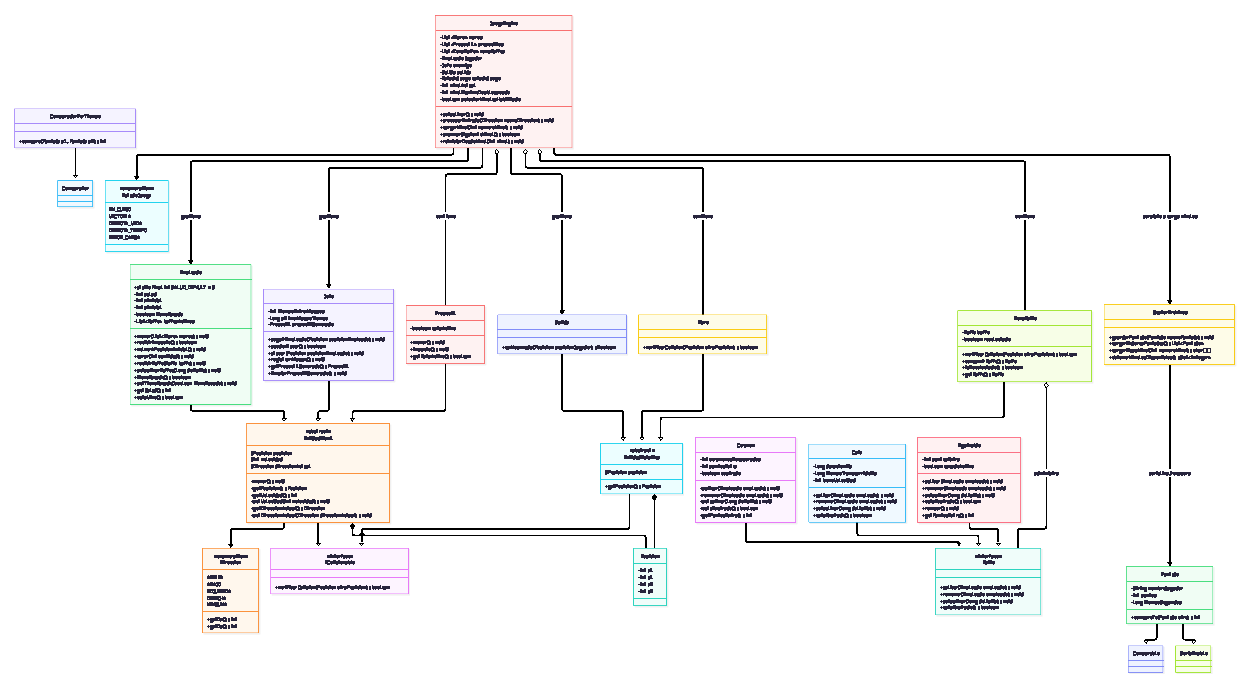
\includegraphics[width=\textwidth]{assets/diagramas/diagrama_clases-1.pdf}
    \caption{Diagrama de Clases UML: Capa de Dominio, Servicios y Controlador de \textit{Escape Corporativo}.}
    \label{fig:uml_dominio}
\end{figure}

\begin{figure}[H]
    \centering
    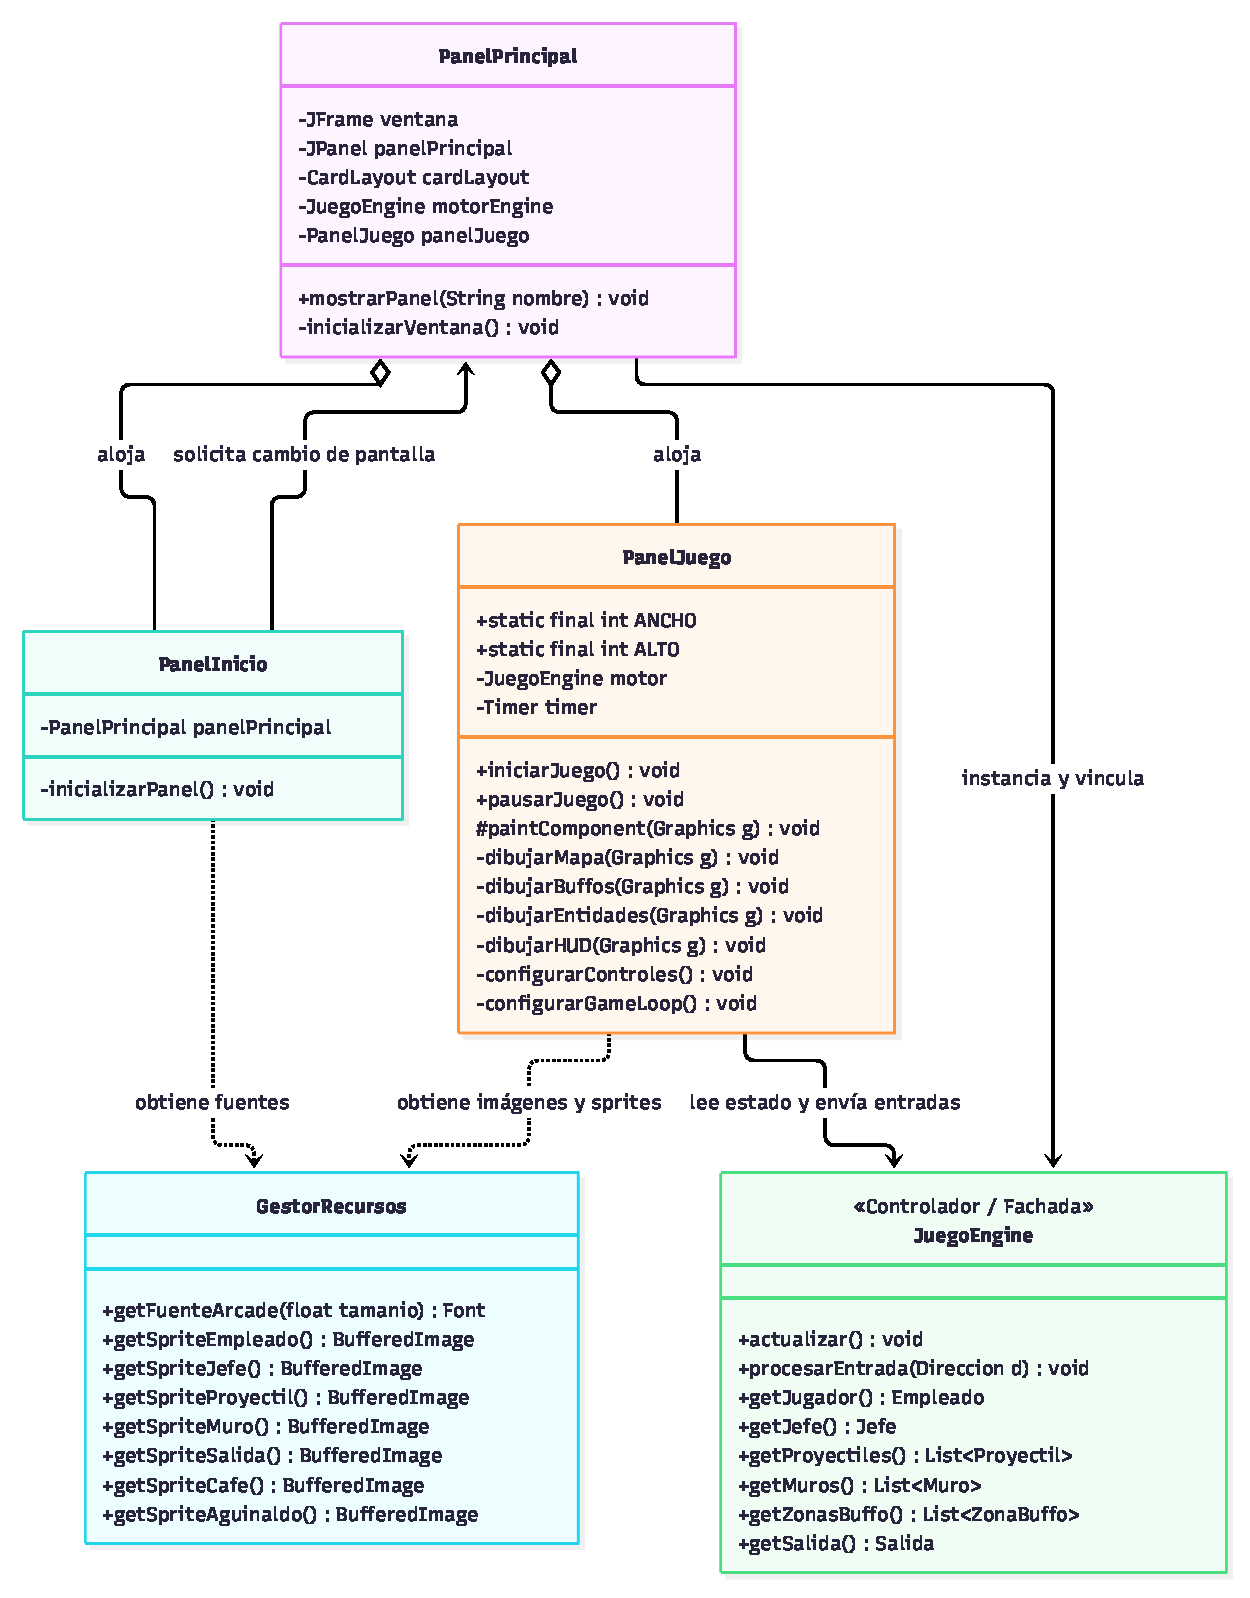
\includegraphics[width=0.88\textwidth]{assets/diagramas/diagrama_clases-2.pdf}
    \caption{Diagrama de Clases UML: Capa de Vista e Interfaz Gráfica (Swing / AWT).}
    \label{fig:uml_vista}
\end{figure}

\begin{figure}[H]
    \centering
    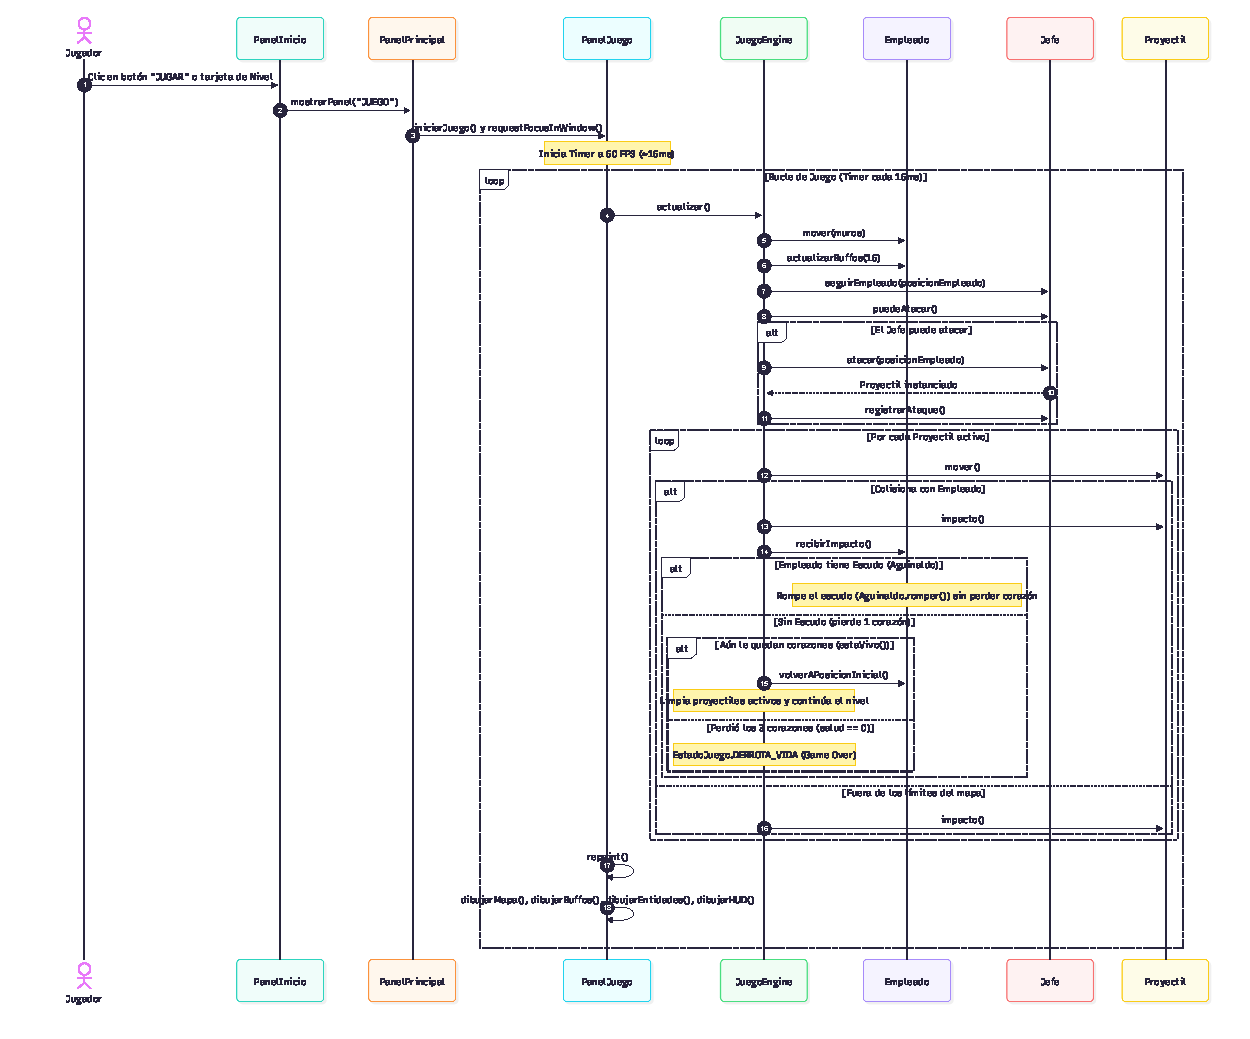
\includegraphics[width=0.95\textwidth]{assets/diagramas/diagrama_clases-3.pdf}
    \caption{Diagrama de Secuencia UML: Ciclo de actualización del \textit{Game Loop}, IA y colisiones balísticas.}
    \label{fig:uml_secuencia}
\end{figure}

\subsection{Descripción de las clases principales}
\begin{itemize}[leftmargin=1.5cm]
    \item \code{EntidadMovil} \textbf{y} \code{EntidadEstatica} \textbf{(Clases Abstractas):} Cimientos de la jerarquía espacial del juego. Centralizan la composición con \code{Posicion} y, en el caso de las entidades móviles, la cinemática vectorial gobernada por \code{Direccion} y \code{velocidad}.
    \item \code{Empleado} \textbf{(Clase Concreta):} Representa al avatar del jugador; administra sus 3 corazones de vida, su escudo activo, su retorno a la coordenada inicial tras impactos (\code{volverAPosicionInicial()}), evalúa colisiones contra muros antes de desplazarse y gestiona el ciclo de vida de su colección polimórfica de \code{Buffo} activos.
    \item \code{Jefe} \textbf{y} \code{Proyectil} \textbf{(Clases Concretas):} El \code{Jefe} ejecuta la lógica de persecución horizontal y cadencia de tiro incremental por nivel, instanciando objetos \code{Proyectil} que se desplazan verticalmente implementando \code{IColisionable}.
    \item \code{ZonaBuffo}, \code{Cafe}, \code{Aguinaldo} \textbf{y} \code{Corazon} \textbf{(Sistema de Ítems):} \code{ZonaBuffo} modela las casillas interactivas del laberinto que contienen una instancia polimórfica de \code{Buffo} (\code{Cafe} para velocidad temporal, \code{Aguinaldo} como escudo protector de 1 impacto y \code{Corazon} para restaurar $+1$ vida).
    \item \code{JuegoEngine} \textbf{(Controlador Principal):} Orquesta el \textit{Game Loop}, procesa las entradas del usuario provenientes de la vista, coordina las colisiones, conserva los corazones entre niveles, administra el desbloqueo progresivo de los 4 mapas y delega la persistencia.
    \item \code{GestorArchivos}, \code{GestorAudio} \textbf{y} \code{GestorRecursos} \textbf{(Servicios y Soporte):} Resuelven respectivamente la serialización del ranking (\code{Puntaje}) y lectura de mapas \texttt{.txt}, la reproducción concurrente de música y SFX en hilos independientes (\code{Runnable}), y el almacenamiento en caché de sprites y fuentes tipográficas.
    \item \code{PanelPrincipal}, \code{PanelInicio}, \code{PanelJuego}, \code{PanelRanking} \textbf{y} \code{PanelVictoria} \textbf{(Capa Vista):} Construyen la interfaz gráfica en Swing utilizando \code{CardLayout}, un diálogo modal personalizado (\code{JDialog}) en \code{PanelInicio} para el selector de niveles con tarjetas de dificultad, y renderizado 2D en tiempo real con HUD de corazones y estado de escudo en \code{PanelJuego}.
\end{itemize}

% ==============================================================================
% 8. ALCANCE Y PLAN DE TRABAJO
% ==============================================================================
\section{Alcance y plan de trabajo}

\indent El desarrollo del proyecto se organizó de forma incremental a lo largo del cuatrimestre, cumpliendo la totalidad de los hitos pautados por la cátedra:

\begin{table}[H]
\centering
\begin{tabularx}{\textwidth}{>{\raggedright\arraybackslash}p{4.0cm} X >{\raggedright\arraybackslash}p{3.2cm}}
\rowcolor{headerbg}
\textbf{Entrega} & \textbf{Contenido previsto} & \textbf{Estado} \\
\hline
Primera entrega & Documento de diseño de juego (GDD) y diagrama de clases UML preliminar. & Completado (05/10/2026) \\
\arrayrulecolor{bordergray}\hline
Segunda entrega & Modelo de dominio en Java: jerarquías de clases abstractas, herencia, enumerados, colecciones genéricas y manejo de excepciones. & Completado (26/10/2026) \\
\hline
Entrega final & Aplicación completa e integrada con interfaz gráfica Swing (\code{CardLayout}), progresión de 4 niveles con selector desbloqueable, sistema de 3 corazones y escudo, ranking con \code{Comparable}/\code{Comparator}, hilos de audio (\code{Runnable}), persistencia binaria y defensa oral. & Completado (16/11/2026) \\
\arrayrulecolor{black}\hline
\end{tabularx}
\end{table}

% ==============================================================================
% 9. CONCLUSIÓN
% ==============================================================================
\newpage
\section{Conclusión}

\indent El proyecto \textbf{ESCAPE CORPORATIVO: LA FUGA DEL EMPLEADO} articula de manera exhaustiva y genuina las exigencias académicas de la asignatura \textit{Paradigma Orientado a Objetos} a través de un videojuego funcional, interactivo y extensible. Mediante la separación de responsabilidades en una arquitectura MVC y la aplicación rigurosa de abstracción, herencia, polimorfismo, contratos por interfaces, principios SOLID y patrones GRASP, se logró construir un código fuente modular y mantenible que integra colecciones genéricas, tratamiento robusto de excepciones propias, concurrencia multihilo y persistencia en disco en un entorno gráfico en tiempo real.

\vspace{0.5cm}
\noindent\textit{Nota: Se utilizó asistencia de herramientas de inteligencia artificial para la revisión de estilo, maquetación en \LaTeX{} y fluidez en la redacción general del documento.}

\end{document}
